\documentclass[aspectratio=169]{beamer}

% ---------- THEME & LOOK ----------
\usetheme{Madrid}
\usecolortheme{seahorse}
\usefonttheme{professionalfonts}
\setbeamertemplate{navigation symbols}{}
\setbeamercovered{transparent}
\setbeamertemplate{itemize items}[circle]
\setbeamertemplate{enumerate items}[default]
\setlength{\parskip}{0.25em}

% ---------- COLORS ----------
\usepackage{xcolor}
\definecolor{accent}{RGB}{0,92,184}
\setbeamercolor{structure}{fg=accent}
\setbeamercolor{title}{fg=white,bg=accent}
\setbeamercolor{frametitle}{fg=accent}
\setbeamercolor{block title}{bg=accent!10,fg=accent}
\setbeamercolor{block body}{bg=accent!3}

% ---------- PACKAGES ----------
\usepackage{booktabs}
\usepackage{amsmath, amssymb}
\usepackage{array}
\usepackage{hyperref}
\hypersetup{colorlinks=true,linkcolor=accent,urlcolor=accent}

% ---------- PLACEHOLDER BOX (compile-safe; no images required) ----------
\newcommand{\placeholderbox}[2][0.82\linewidth]{%
  \begin{center}
    \fbox{\begin{minipage}[c][0.46\textheight][c]{#1}
      \centering \vspace{0.25em}
      \textbf{#2}\\[0.6em]
      \emph{Insert figure/diagram here later.}
    \end{minipage}}
  \end{center}
}

% ---------- TITLE ----------
\title{\textbf{Wages and Employment in a Single Labour Market\vspace{.5cm}\\  }}
\subtitle{ {\large ECON 300 - Labour Economics}}
%\institute{UNBC}
\author{Muhebullah Karimzada}

\date{Winter 2026}



\begin{document}

% ============================================================
% TITLE
% ============================================================
\begin{frame}[plain]
  \titlepage

\end{frame}


\begin{frame}{Learning Objectives}
\transfade
\begin{itemize}[<+->]
  \item Construct market supply and demand and compute equilibrium wage and employment.
  \item Contrast competitive outcomes with imperfect competition (monopoly, oligopoly, monopolistic competition).
  \item Explain how monopsony reduces wages and employment relative to competition.

\end{itemize}
\end{frame}

\begin{frame}{Main Questions}
\transfade
\begin{itemize}[<+->]
  \item How are wages and employment determined in a single labour market?
  \item How does imperfect competition modify the supply-demand analysis?
  \item Who bears payroll taxes -- workers or firms?
  \item What is monopsony? How different are outcomes when firms have hiring power?
\end{itemize}
\end{frame}



% ============================================================
\section{Competitive Interaction with Markets}
% ============================================================

\begin{frame}{The Competitive Firm’s Interaction with the Market}
\transfade
\begin{itemize}[<+->]
  \item Competitive in both product and labour markets
  \item Homogeneous labour; firm is a price and wage taker
  \item Firm can hire all needed labour at the market wage
  \item Market wage set by aggregate labour market
\end{itemize}
\end{frame}

\begin{frame}{Figure 7.1: Competitive Product and Labour Markets}
\centering
\vspace{2em}

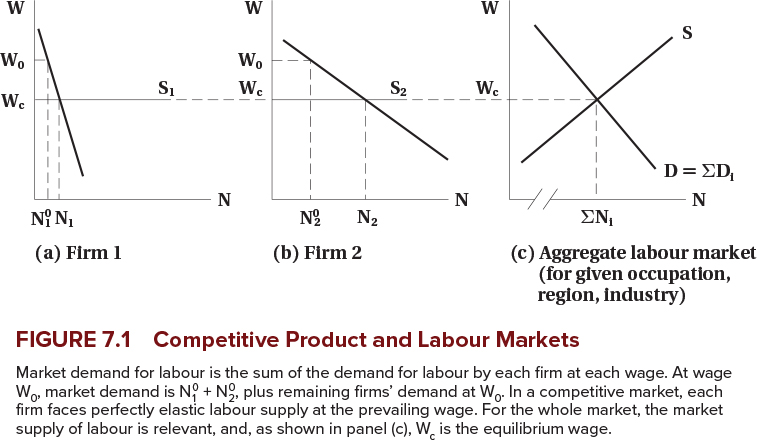
\includegraphics[width=1.02\linewidth]{ben54842_0701}
\end{frame}

\begin{frame}{Panels (a) and (b): Individual Firm Labour Demand}
\textbf{Firm Labour Demand}
\begin{itemize}
\item Downward-sloping curve = \textbf{value of marginal product of labour (VMPL)}
\item Hiring rule:
\[
\text{Hire labour until } VMPL = W
\]
\item Each firm faces a \textbf{perfectly elastic labour supply} at the market wage
\end{itemize}

\textbf{Effect of a Wage Change}
\begin{itemize}
\item At wage $W_0$, Firm $i$ hires $N_i^0$
\item At lower wage $W_c$, labour hired increases to $N_i$
\item Firms hire more labour when wages fall
\end{itemize}

\textbf{Key Insight}
\begin{itemize}
\item Individual firms take wages as given
\item Labour demand responds to wage changes
\end{itemize}
\end{frame}

\begin{frame}{Panel (c): Aggregate Labour Market}
\textbf{Market Labour Demand}
\begin{itemize}
\item Market demand is the \textbf{horizontal sum} of firm demands:
\[
D = \sum_i D_i
\]
\item At wage $W_0$:
\[
N^{market} = N_1^0 + N_2^0 + \cdots
\]
\end{itemize}

\textbf{Labour Supply}
\begin{itemize}
\item Upward-sloping curve $S$ represents market labour supply
\end{itemize}

\textbf{Equilibrium}
\begin{itemize}
\item Wage $W_c$ clears the market
\item Labour supply equals labour demand
\item Firms hire where $W_c = VMPL$
\end{itemize}
\end{frame}


\begin{frame}{Labour Supply in Figure 7.1}
\textbf{Labour Supply at the Firm Level (Panels a \& b)}
\begin{itemize}
\item Each firm faces a \textbf{perfectly elastic labour supply} at the market wage
\item Represented by horizontal lines ($S_1$, $S_2$)
\item Reason:
\begin{itemize}
\item Individual firms are wage takers
\item They can hire as many workers as desired at the prevailing wage
\item Hiring decisions do \emph{not} affect the wage
\end{itemize}
\end{itemize}

\vspace{0.3cm}

\textbf{Labour Supply in the Market (Panel c)}
\begin{itemize}
\item Market labour supply curve ($S$) is \textbf{upward sloping}
\item Reflects workers’ willingness to supply more labour at higher wages
\item Determined by:
\begin{itemize}
\item worker preferences (income vs leisure)
\item alternative employment opportunities
\item demographics and participation decisions
\end{itemize}
\end{itemize}

\end{frame}


\begin{frame}{Short Run vs.\ Long Run to the Firm}
\transfade
\begin{itemize}[<+->]
  \item Short run: Product demand rise \(\Rightarrow\) higher labour demand; wage and employment rise (given upward-sloping supply to the firm).
  \item Long run: Higher short-run wages attract more workers; labour supply shifts right; wage adjusts.
\end{itemize}
\end{frame}

\begin{frame}{Figure 7.2: Short-Run and Long-Run Labour Supply Schedules }
\centering
\vspace{2em}

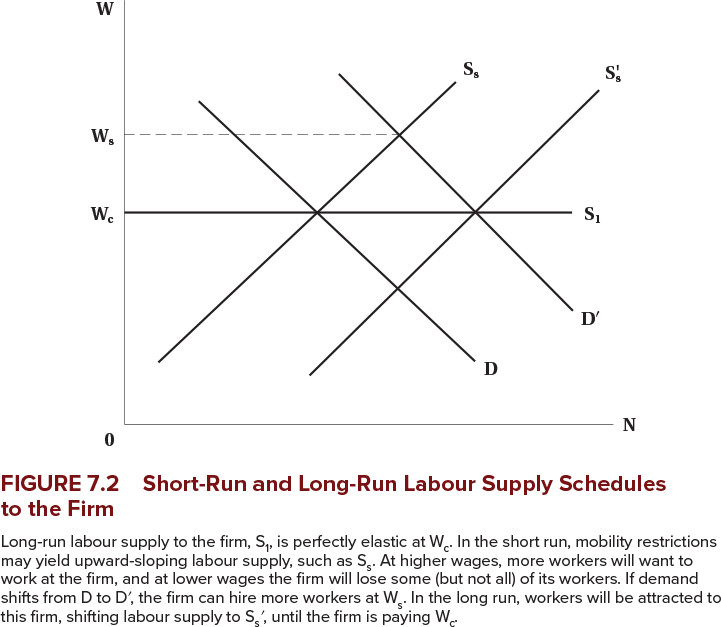
\includegraphics[width=.7\linewidth]{ben54842_0702}
\end{frame}

\begin{frame}{Competitive Equilibrium}
\transfade
\textbf{Short-run:}
\begin{itemize}[<+->]
\item Even a competitive firm may have to raise its wages to attract  additional workers
\begin{itemize}
\item dynamic monopsony
\end{itemize}
\item The firm's short-run labour supply schedule could be upward sloping, $S_{s}$
\end{itemize}

\textbf{Long-run:}
\begin{itemize}[<+->]
\item Since $W_{s}>W_{c}$ $\Rightarrow$ there will be supply influx of additional workers
\item Resulting in the shift of supply schedule from $S_{s}$ to $S^{'}_{s}$
\item The supply influx would depress the temporarily high, short-run wage of $W_{s}$ back to its long-run level of $W_{c}$
\end{itemize}
\end{frame}

% ============================================================
\section{Imperfect Competition in Product Markets}
% ============================================================

\begin{frame}{Monopoly: Effects of Hiring More Labour}
\transfade
\begin{itemize}[<+->]
  \item \(MPP_N \downarrow\) with more \(N\)
  \item \(MR\) falls as more output sold requires lower price
  \item Labour demand under monopoly \(<\) under competition
\end{itemize}
\end{frame}

\begin{frame}{Figure 7.3: Monopolist vs.\ Competitive Demand for Labour }
\centering
\vspace{2em}

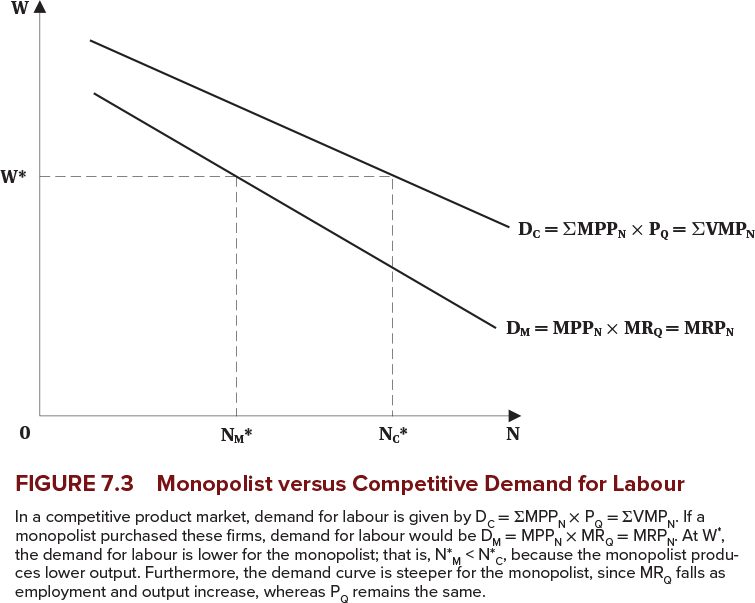
\includegraphics[width=0.71\linewidth]{ben54842_0703}
\end{frame}

\begin{frame}{Figure 7.3: Monopolist vs Competitive Demand for Labour}

\textbf{Competitive Labour Demand ($D_C$)}
\begin{itemize}
\item Firms are price takers in the product market
\item Output price is constant: $P_Q$
\item Labour demand equals the \textbf{value of marginal product}:
\[
D_C = VMP_N = MPP_N \times P_Q
\]
\item Higher employment level: $N_C^*$
\end{itemize}

\textbf{Monopolist Labour Demand ($D_M$)}
\begin{itemize}

\item Marginal revenue is less than price: $MR_Q < P_Q$
\item Labour demand equals the \textbf{marginal revenue product}:
\[
D_M = MRP_N = MPP_N \times MR_Q
\]
\item Curve lies below $D_C$ and is steeper -- $MR_Q$ falls as employment and output increase
\item Lower employment level: $N_M^*$
\end{itemize}

\end{frame}



\begin{frame}{Oligopoly \& Monopolistic Competition}
\transfade
\begin{itemize}[<+->]
  \item Oligopoly: few firms; strategic interdependence
  \item Possible departures from market wages (above-normal profits may be partly shared)
  \item Monopolistic competition: short-run profits \(\Rightarrow\) possibly higher-than-market wages; long-run zero profit \(\Rightarrow\) market wages
\end{itemize}
\end{frame}



% ============================================================
\section{Working with Supply and Demand}
% ============================================================

\begin{frame}{Linear Supply and Demand: Setup}
\transfade
\small
\[
N_D = a + b\,W; b<0,\qquad N_S = c + f\,W; f>0
\]

\vspace{0.7cm}

Setting \(N_S=N_D\) yields equilibrium \((w^\ast,N^\ast)\).
\medskip

\textbf{With Shifter \(z\):}
\[
N_D = a + b\,w + \gamma z,\qquad N_D = c - d\,w + \delta z
\]
Solve again for new \((w^\ast,N^\ast)\) to study incidence and comparative statics.
\end{frame}

\begin{frame}{Figure 7.4: Linear Supply and Demand }
\centering
\vspace{2em}

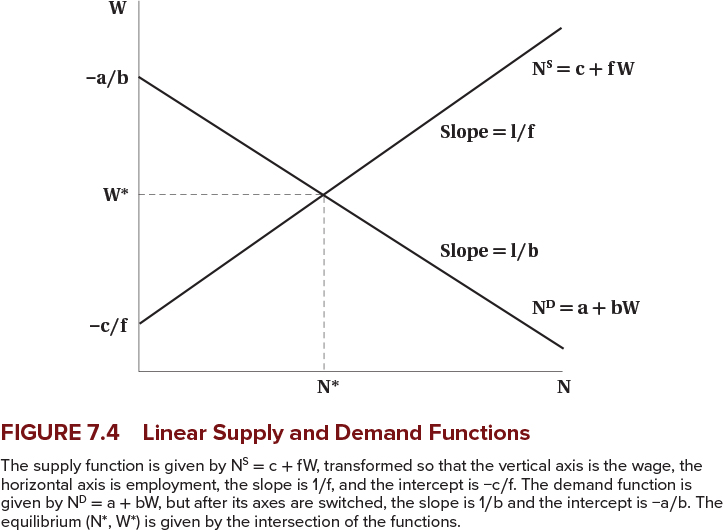
\includegraphics[width=0.79\linewidth]{ben54842_0704}
\end{frame}

% ============================================================
\section{Payroll Taxes: Application}
% ============================================================

\begin{frame}{Application: Incidence of a Unit Payroll Tax}
\transfade
\begin{itemize}[<+->]
  \item Examples: CPP/QPP, workers’ compensation, EI, health/education payroll levies
  \item Often called “job killers” — but actual incidence depends on elasticities
\end{itemize}
\end{frame}

\begin{frame}{TABLE 7.1: Payroll Taxes as a Percentage of Labour Income, Canada (1971, 1997)}
\transfade
\small
\begin{tabular}{lcc}
\toprule
\textbf{Type of Payroll Tax} & \textbf{1971} & \textbf{1997} \\
\midrule
Workers’ compensation & 0.73 & 1.61 \\
Unemployment insurance & 1.06 & 4.98 \\
Canada/Quebec pension & 2.12 & 3.92 \\
Health and/or education & 0.21 & 1.71 \\
\textbf{Total} & \textbf{4.12} & \textbf{12.23} \\
\bottomrule
\end{tabular}
\end{frame}

\begin{frame}{Payroll Tax in the Model}
\transfade
\small
Let a per-worker tax \(t\) on firms shift the perceived cost:
\[
N_D = c - d(w+t)
\]
Incidence on wages vs.\ employment depends on the elasticities of \(N_S\) and \(N_D\).
\end{frame}

\begin{frame}{Figure 7.5: Effect of a Payroll Tax on Employment and Wages}
\centering
\vspace{2em}

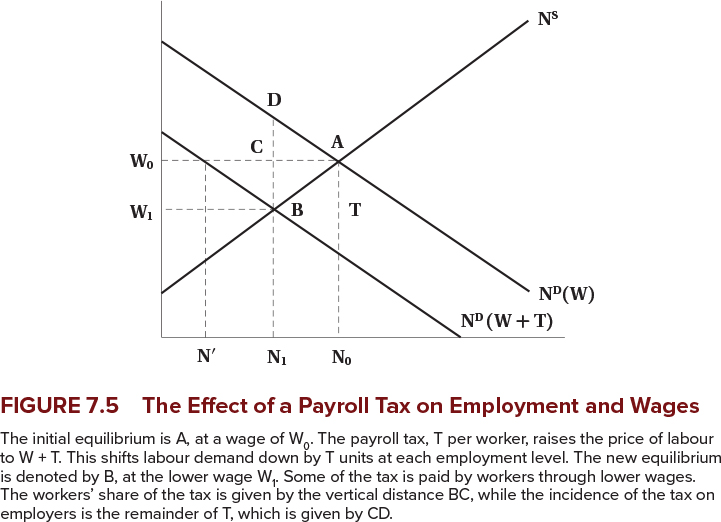
\includegraphics[width=0.85\linewidth]{ben54842_0705}
\end{frame}


\begin{frame}{Figure 7.5: Payroll Tax, Wages, and Employment}

\textbf{Initial Equilibrium}
\begin{itemize}
\item Labour supply: $N^S$
\item Labour demand: $N^D(W)$
\item Initial equilibrium at point $A$
\item Wage = $W_0$, Employment = $N_0$
\end{itemize}

\textbf{Introduction of a Payroll Tax ($T$ per worker)}
\begin{itemize}
\item Tax raises cost of labour to employers to $W + T$
\item Labour demand shifts downward to $N^D(W+T)$
\item New equilibrium at point $B$
\item Workers receive lower wage: $W_1$
\item Employment falls from $N_0$ to $N_1$
\end{itemize}



\end{frame}

\begin{frame}{Figure 7.5: Payroll Tax, Wages, and Employment}


\textbf{Tax Incidence}
\begin{itemize}
\item Total tax per worker = $T$
\item Workers bear part of the burden:
\[
\text{Worker share} = BC
\]
\item Employers bear the remainder:
\[
\text{Employer share} = CD
\]
\end{itemize}

\textbf{Summary}
\begin{itemize}
\item Payroll taxes reduce employment and wages
\item Tax burden is shared between workers and firms
\item The side of the market that is less elastic bears more of the tax burden
\end{itemize}

\end{frame}



% ============================================================
\section{Monopsony in the Labour Market}
% ============================================================

\begin{frame}{Monopsony: Basics}
\transfade
\begin{itemize}[<+->]
\item  A monopsony is a labour market with one dominant firm.
  \item Large firm relative to labour market size; influences wage

\item It faces an upward-sloping labour supply curve 

\item To hire more workers, the firm must offer higher wages.
  \item Marginal cost of labour exceeds average cost (wage) due to\textbf{ inframarginal uprating}
\end{itemize}

 \textbf{Inframarginal uprating} is an increase in benefit levels for individuals already eligible for a program.
\begin{itemize}[<+->]
\item Eligibility rules remain unchanged.

\item Raises payments to current recipients
\item Does not expand eligibility
\item Does not directly add new participants
\end{itemize}
\end{frame}

 \begin{frame}{Inframarginal Uprating}




\textbf{Example}
\begin{itemize}
\item Unemployment benefits increase from \$500 to \$550 per week for current recipients.
\end{itemize}

\textbf{Economic Effects}
\begin{itemize}
\item Increases recipients’ income
\item May reduce labour supply through an income effect
\item Participation incentives at eligibility thresholds remain unchanged
\end{itemize}

\textbf{Contrast}
\begin{itemize}
\item \textbf{Marginal reform:} A policy that expands eligibility or lowers the cutoff -- affects marginal entrants, not inframarginal recipients.
\end{itemize}

\end{frame}

\begin{frame}{Figure 7.6: Monopsony }
\centering
\vspace{2em}

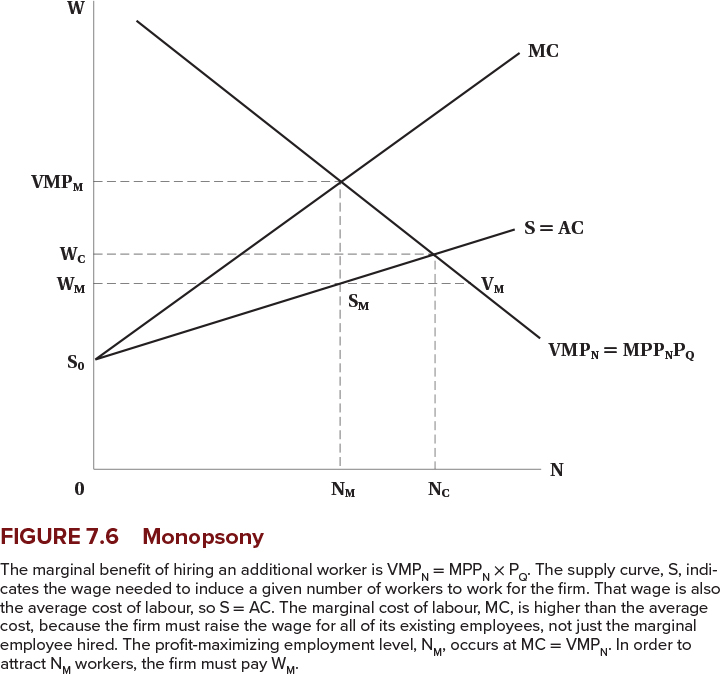
\includegraphics[width=0.63\linewidth]{ben54842_0706}
\end{frame}


\begin{frame}{Figure 7.6: Monopsony in the Labour Market}

\textbf{Curves in the Figure}
\begin{itemize}
\item Labour supply ($S = AC$): wage required to attract workers; also the average cost of labour.
\item Marginal cost of labour ($MC$): lies above supply since hiring one more worker requires raising wages for all workers.
\item Labour demand ($VMP_N$):
\[
VMP_N = MPP_N \times P_Q
\]
downward sloping due to diminishing productivity.
\end{itemize}

\textbf{Monopsony Outcome}
\begin{itemize}
\item Profit maximization occurs where $MC = VMP_N$.
\item Employment: $N_M$
\item Wage paid: $W_M$ (from the supply curve)
\end{itemize}
\end{frame}

\begin{frame}{Figure 7.6: Monopsony in the Labour Market}
\textbf{Competitive Benchmark}
\begin{itemize}
\item Competitive equilibrium: $N_C$ and $W_C$
\item Monopsony results:
\[
N_M < N_C \quad \text{and} \quad W_M < W_C
\]
\end{itemize}

\textbf{Key Point}
\begin{itemize}
\item Market power allows the firm to restrict employment and suppress wages.
\end{itemize}

\end{frame}

\begin{frame}{Perfect Monopsonistic Wage Differentiation}

\textbf{Definition}
\begin{itemize}[<+->]
\item Occurs when a monopsonist pays each worker a wage equal to their \textbf{reservation wage}.
\item The firm has full information about workers’ minimum willingness to work.
\item Workers receive different wages instead of a single uniform wage.
\end{itemize}

\textbf{Key Mechanism}
\begin{itemize}[<+->]
\item Hiring an additional worker does \emph{not} require raising wages for existing workers.
\item The labour supply curve becomes the firm's marginal cost of labour:
\[
MC = \text{Labour Supply}
\]
\end{itemize}

\textbf{Hiring Rule}
\begin{itemize}[<+->]
\item The firm hires labour where:
\[
VMP_N = \text{Labour Supply}
\]
\end{itemize}

\end{frame}

\begin{frame}{Implications of Wage Differentiation}

\textbf{Employment Outcome}
\begin{itemize}
\item Employment equals the competitive level.
\item The efficient number of workers is hired.
\end{itemize}

\textbf{Distribution of Surplus}
\begin{itemize}
\item Workers receive wages equal to their reservation wages.
\item Worker economic rent (the surplus income a worker receives above their reservation wage) is eliminated.
\item The firm captures all surplus.
\end{itemize}
\end{frame}



\begin{frame}{Implications of Wage Differentiation}
\textbf{Comparison}
\begin{itemize}
\item Competitive market: single wage, surplus shared.
\item Single-wage monopsony: lower wage, reduced employment.
\item Perfect wage discrimination: efficient employment, firm captures surplus.
\end{itemize}

\textbf{Real-World Relevance}
\begin{itemize}
\item Pure wage discrimination is rare.
\item Partial forms appear through:
\begin{itemize}
\item individualized contracts
\item performance pay
\item bargaining and bonuses
\item non-wage compensation
\end{itemize}
\end{itemize}

\end{frame}









\begin{frame}{Summary}
\transfade
\begin{itemize}[<+->]
  \item Competitive equilibrium determines wage and employment; product market power lowers labour demand.
  \item Payroll tax incidence depends on elasticities; wages and employment adjust accordingly.
  \item Monopsony lowers wage and employment; targeted minimum wage can raise both.
  \item Measuring minimum wage effects empirically remains contested.
\end{itemize}
\end{frame}

% ============================================================
\begin{frame}
\centering
\Huge{\textbf{Thank You!}} \\

\end{frame}

\end{document}
